\documentclass{report}

\usepackage{amsmath, amssymb, amsfonts}
%\usepackage{pdfsync}
\usepackage{graphicx,subcaption,verbatim}
%\usepackage{fancyhdr}

\usepackage{tikz}
\usepackage[forpaper, 
useforms , %nosolutions, pointsonleft
nopoints,answerkey
]{eqexam}

\usetikzlibrary{calc,arrows,decorations.markings,shapes.geometric}
%\usepackage[usenames]{color}
%\definecolor{myblue}{rgb}{.2, .2, .7}

\usepackage{pgfplots}
\pgfplotsset{compat=newest}



\newcommand\dsp{\displaystyle}

\newcommand{\norm}[1]{\left\Vert #1 \right\Vert}
\newcommand{\avec}[1]{\left\langle #1 \right\rangle}
\newcommand{\Reals}{\mathbb{R}}
\newcommand{\vect}[1]{\overrightarrow{#1}}
\newcommand{\abs}[1]{\left\vert{#1}\right\vert}

\rheadeqe{} % no name on pages other than first



\title[MT1]{Midterm Exam 1} %\author{O. Bastille}
\subject{MATH253X-UX1} 
\examNameLabel{Name:}
%\date{\thisterm\space\the\year}
\date{Spring 2016}
\chead{-- Page \arabic{page}\space of \eqExamLastPage\space--}

\begin{document}\maketitle

% Formal beginning of the exam.
\begin{exam}{Part1}
\begin{instructions}
You have 60 minutes. No notes, book, or calculators allowed. \emph{Show all your work} in order to receive full credit.
\end{instructions}

%-------------------------------Problem 1------------------------------
\begin{problem*}[\auto] Consider a triangle in space with vertices $A(1,0,-1)$, $B(2,2,-2)$, and $C(-2,1,0)$.


\begin{parts}
	\item\PTs{3} Find the equation of the sphere centered at $A$ and going through $B$.
	\begin{solution}[1in]
	Radius of the sphere: $\norm{\vect{AB}}= \sqrt{(2-1)^2+(2-0)^2+(-2+1)^2}=\sqrt{1+4+1}=\sqrt{6}$. So the equation of the sphere is:
	$$\boxed{(x-1)^2+y^2+(z+1)^2=6}. $$
		\end{solution}
		\item\PTs{5} Find the cosine of the angle at vertex $A$ in the triangle.
		\begin{solution}[1.5in]\begin{align*}
		\cos \alpha &= \dfrac{\vect{AB}\cdot\vect{AC}}{\norm{\vect{AB}}\norm{\vect{AC}}}=\frac{\avec{2-1,2-0,-2+1}\cdot\avec{-2-1,1-0,0+1}}{\sqrt{6}\sqrt{(-2-1)^2+(1-0)^2+(0+1)^2}}\\
		&=\frac{\avec{1,2,-1}\cdot\avec{-3,1,1}}{\sqrt{6}\sqrt{9+1+1}}=\frac{1(-3)+2(1)-1(1)}{\sqrt{6}\sqrt{11}}\\
		&=\frac{-2}{\sqrt{66}}=\boxed{-\frac{\sqrt{66}}{33}}
		\end{align*}
		\end{solution}
\item\PTs{8} Find the equation of the plane containing the triangle $ABC$.
\begin{solution}[1.75in] A normal vector to the plane is (any scalar multiple of):
$$\vect{AB}\times\vect{AC}=\begin{vmatrix}\mathbf{i} & \mathbf{j} & \mathbf{k}\\
1& 2 & -1\\
-3 & 1 & 1 \end{vmatrix}=\avec{2(1)-1(-1),-(1(1)+3(-1)),1(1)+3(2)}=\avec{3,2,7}. $$
And so the equation of the plane is:
$$\boxed{3(x-1)+2y+7(z+1)=0} \quad\text{ or equivalently }\quad\boxed{3x+2y+7z+4=0}.$$
\end{solution}

\end{parts}
\end{problem*}

%---------------------------Problem 2------------------------------
\begin{problem*}[\auto] Let $\mathbf{r}(t)=\avec{3\cos t,5 \sin t,-4 \cos t}$ describe the trajectory of a particle over time, where position is measured in meters and time in seconds. 
	\begin{parts}
		\item\PTs{6} Find the distance traveled (i.e. the arc length) from $t=0$ s to $t=2\pi$ s.
		\begin{solution}[2in] We have:
		\begin{align*}
		\mathbf{r}'(t)&=\avec{-3\sin t,5 \cos t,4\sin t}\\
		\quad\Rightarrow\quad \norm{\mathbf{r'}(t)}&=\sqrt{9\sin^2t+25\cos^2t+16\sin^2t}=\sqrt{25\sin^2t+25\cos^2t}=\sqrt{25}=5 \text{ m/s}.
		\end{align*}
		So the distance traveled is:
		$$s=\int_{0}^{2\pi}\norm{\mathbf{r'}(t)}\;dt=\int_0^{2\pi}5\;dt=\Big[5t\Big]_{0}^{2\pi}=\boxed{10\pi\text{ m}}. $$
		\end{solution}
		\item\PTs{4} Show that the trajectory $\mathbf{r}(t)=\avec{3\cos t,5 \sin t,-4 \cos t}$ sits on both surfaces $4x+3z=0$ and $\dfrac{x^2}{9}+\dfrac{y^2}{25}=1$ at all times.
		\begin{solution}[2.2in] Since $x=3\cos t$, $y=5\sin t$, and $z=-4\cos t$, then for all $t$:
		$$4x+3z=4(3\cos t)+3(-4\cos t)=12\cos t-12 \cos t=0 \quad \text{\checkmark}$$
		and
		$$\dfrac{x^2}{9}+\dfrac{y^2}{25}=\frac{(3\cos t)^2}{9}+\dfrac{(5\sin t)^2}{25}=\frac{9\cos^2t}{9}+\frac{25\sin^2t}{25}=\cos^2t+\sin^2t=1\quad \text{\checkmark} $$
		\end{solution}
		\item\PTs{6} Sketch the surface $\dfrac{x^2}{9}+\dfrac{y^2}{25}=1$. Include a scale. 
		\begin{solution}[2.5in]
		\begin{center}
			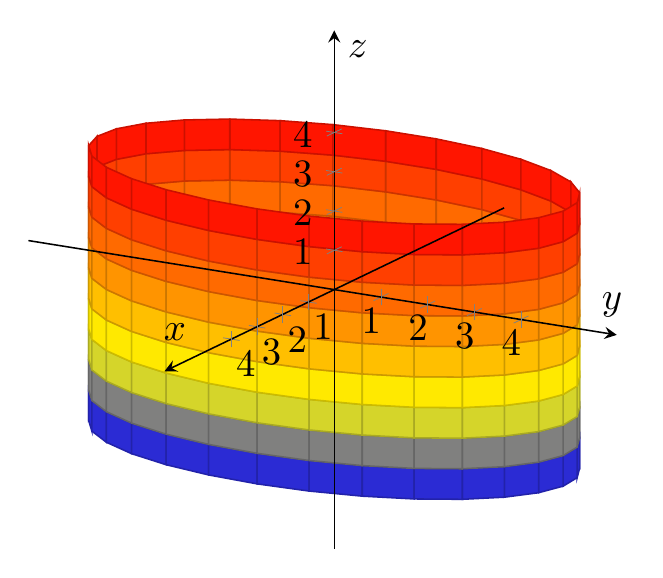
\begin{tikzpicture}[scale=1.4]
						\begin{axis}[
						width=10cm, view={120}{20},
						axis on top,
						axis lines=center,
						enlargelimits=.1,
						ymin=-5.5, ymax=5, xmin=-5.5, xmax=5.5, zmin=-5.5, zmax=5.5,
						xlabel=$x$, ylabel=$y$, zlabel=$z$, xtick={1,2,3,4},ytick={1,2,3,4},ztick={1,2,3,4}
						]
						\addplot3[surf,domain=0:360,y domain=-4:3,samples=30,samples y=10,z buffer=sort] ({3*cos(x)},{5*sin(x)},y);
						\end{axis}
						\end{tikzpicture}
						\end{center}
		\end{solution}
		\begin{workarea}{2.5in}
\begin{center}
	\begin{tikzpicture}[scale=1.4]
				\begin{axis}[
				width=10cm, view={120}{20},
				axis on top,
				axis lines=center,
				enlargelimits=.1,
				ymin=-5.5, ymax=5, xmin=-5.5, xmax=5.5, zmin=-5.5, zmax=5.5,
				xlabel=$x$, ylabel=$y$, zlabel=$z$, xtick=\empty,ytick=\empty,ztick=\empty
				]
				\end{axis}
				\end{tikzpicture}
\end{center}
\end{workarea}	
		\end{parts}
	
	\end{problem*}
	
	%------------------Problem 3----------------------
	\begin{problem*}[\auto] Consider vectors $\mathbf{a}$ and $\mathbf{b}$ as shown below.
		\begin{parts}
			\item\PTs{4} Sketch the following:
\begin{solution}[1.75in]			
		\vskip0.2in
			\begin{tikzpicture}
			\tikzset{
			    right angle quadrant/.code={
			        \pgfmathsetmacro\quadranta{{1,1,-1,-1}[#1-1]}     % Arrays for selecting quadrant
			        \pgfmathsetmacro\quadrantb{{1,-1,-1,1}[#1-1]}},
			    right angle quadrant=1, % Make sure it is set, even if not called explicitly
			    right angle length/.code={\def\rightanglelength{#1}},   % Length of symbol
			    right angle length=0.5ex, % Make sure it is set...
			    right angle symbol/.style n args={3}{
			        insert path={
			            let \p0 = ($(#1)!(#3)!(#2)$),     % Intersection
			                \p1 = ($(\p0)!\quadranta*\rightanglelength!(#3)$), % Point on base line
			                \p2 = ($(\p0)!\quadrantb*\rightanglelength!(#2)$), % Point on perpendicular line
			                \p3 = ($(\p1)+(\p2)-(\p0)$) in  % Corner point of symbol
			            (\p1) -- (\p3) -- (\p2)
			        }}}
			\begin{scope}[rotate=15]
			\coordinate (o) at (0,0);
			\coordinate (a) at (3,0);
			\coordinate (b) at (120:1cm);
			\draw[-stealth] (o) -- node[below] {$\mathbf{a}$} (a);
			\draw[-stealth] (o) -- node[below left] {$\mathbf{b}$} (b);
			\draw[blue,ultra thick,-latex] (120:1cm) -- (3,0);
			\end{scope}
			\draw (0,2) node {$\mathbf{a}-\mathbf{b}$};
			\begin{scope}[xshift=10cm]
			\begin{scope}[rotate=15]
				\coordinate (o) at (0,0);
						\coordinate (a) at (3,0);
						\coordinate (b) at (120:1cm);
			\draw[-stealth] (o) -- node[below] {$\mathbf{a}$} (a);
			\draw[-stealth] (o) -- node[below left] {$\mathbf{b}$} (b);
			\coordinate (pba) at ($(o)!(a)!(b)$);
			\draw[very thin,blue,right angle quadrant=1,right angle length=0.15cm,right angle symbol={o}{b}{a}] (pba) -- (a);
			\draw[ultra thick,-latex,blue] (o) -- (pba);
		%cheat, not quite right so use right angle quadrant code from web instead
		%	\coordinate (pbao) at ($(pba)!0.1!(3,0)$);
		%	\coordinate (pbaa) at ($(pba)!0.09!(0,0)$);
		%	\draw[thin,blue] (pbao) -- +(120:0.11cm) -- (pbaa);
		 
			\end{scope}
			\draw (0,2) node {	$ \operatorname{proj}_{\mathbf{b}}\mathbf{a}$};
			 
			\end{scope}
			\end{tikzpicture}

\end{solution}			
				\begin{workarea}{1.75in}
				\vskip0.2in
							\begin{tikzpicture}
							\begin{scope}[rotate=15]
							\draw[-stealth] (0,0) -- node[below] {$\mathbf{a}$} (3,0);
							\draw[-stealth] (0,0) -- node[below left] {$\mathbf{b}$} (120:1cm);
							\end{scope}
							\draw (0,2) node {$\mathbf{a}-\mathbf{b}$};
							\begin{scope}[xshift=10cm]
							\begin{scope}[rotate=15]
							\draw[-stealth] (0,0) -- node[below] {$\mathbf{a}$} (3,0);
							\draw[-stealth] (0,0) -- node[below left] {$\mathbf{b}$} (120:1cm);
							\end{scope}
							\draw (0,2) node {	$ \operatorname{proj}_{\mathbf{b}}\mathbf{a}$};
							\end{scope}
							\end{tikzpicture}
							\vskip0.2in
				\end{workarea}	
		
			\item\PTs{4} State whether the following statements are true or false. Briefly justify.
			\vskip0.2in 
			\begin{itemize}
				\item $\mathbf{a}\cdot\mathbf{b} \ge 0\quad$\fillin[b]{5in}{False. The angle between them is obtuse so cosine is negative.}
				\vskip0.2in
				\item $\mathbf{a}\times\mathbf{b}$ points out of the page towards you. \fillin[b]{3in}{True, by the right hand rule.}
			\end{itemize}
			\end{parts}
		\end{problem*}




%-------------------------------Problem 4-------------------------

\begin{problem*}[\auto]Let a space curve be described by $\mathbf{r}(t)=t\mathbf{i}+t^2\mathbf{j}+3t\mathbf{k}$. 
\begin{parts}
\item\PTs{8} Find the symmetric equations of the tangent line to the curve at the point $P(-1,1,-3)$.
\begin{solution}[1.75in]
\begin{itemize}
\item $\vect{OP}=\mathbf{r}(-1)$
\item $\mathbf{v}(t)=\mathbf{r'}(t)=\avec{1,2t,3}$
\item $\mathbf{v}(-1)=\mathbf{r'}(-1)=\avec{1,-2,3}$
\item so symmetric equations for the tangent line are:
$$\boxed{x+1=\frac{y-1}{-2}=\frac{z+3}{3}} $$
\end{itemize}
\end{solution}
\item\PTs{6} Find the tangential component of the acceleration for any $t$.
\begin{solution}[1.75in] We have
$$\norm{\mathbf{v}(t)}=\sqrt{1+4t^2+9}=\sqrt{4t^2+10} $$
so the tangential component of acceleration is:
$$a_{\mathbf{T}}=\norm{\mathbf{v}}'=\boxed{\frac{4t}{\sqrt{4t^2+10}}}. $$
Or using another form:
$$a_{\mathbf{T}}=\mathbf{a}\cdot\mathbf{T}=\frac{\mathbf{a}\cdot\mathbf{v}}{\norm{\mathbf{v}}}=\frac{\avec{0,2,0}\cdot\avec{1,2t,3}}{\sqrt{4t^2+10}}=\boxed{\frac{4t}{\sqrt{4t^2+10}}} $$
\end{solution}
\end{parts}
\end{problem*}

%----- Problem 4------------------------
\begin{problem*}[\auto] Consider the line given by:
	$$x=2+t\qquad,\qquad y=1-t\qquad,\qquad z=5-4t. $$
	\begin{parts}
		\item\PTs{5} Show that the line is parallel to but not in the plane $x-3y+z=1$.
		\begin{solution}[2in] The line is parallel to the plane if its direction is orthogonal to the normal vector. Here:
		$$\avec{1,-1,-4}\cdot\avec{1,-3,1}=1(1)-1(-3)-4(1)=1+3-4=0 \quad \text{\checkmark} $$
		To show it's not in the plane, we need only one point from the line (since parallel already) to plug into the equation of the plane:
		$$2-3(1)+5=4 \ne 1. $$
		Or from the start, you can plug in the coordinates for the whole line into the plane:
		$$(2+t)-3(1-t)+(5-4t)=2+t-3+3t+5-4t=4 \ne 1 $$
		for any $t$ so there is no intersection between the line and the plane, which will only happen if the line is parallel to the plane but not in it.
		\end{solution}
		\item\PTs{5} Find the distance from the line to the plane. \emph{Hint: } You can use any point from the line.
			\begin{solution}[1.25in] Rewrite the plane as $x-3y+z-1=0$, then using the point $(2,1,5)$ from the line, the distance from the line to the plane is:
			$$d=\dfrac{\abs{2-3(1)+5-1}}{\norm{\avec{1,-3,1}}}=\frac{3}{\sqrt{1+9+1}}=\boxed{\frac{3\sqrt{11}}{11}}. $$
			\end{solution}
		\end{parts}
		\end{problem*}
		
%---------------------------Problem 4--------------------------
\begin{problem*}[\auto] Identify the surface from its equation then sketch the surface. 
	
	\begin{parts}
		\item\PTs{6} $z=1+x^2+\dfrac{y^2}{4}\quad$ 
		\begin{solution}[1.75in]
			
			Type of surface: \underline{$\quad\qquad$ elliptic paraboloid $\quad\qquad$}  % % cheap hack; won't do \hfill in solutions (ok in workarea)
			\hspace{3.5cm} 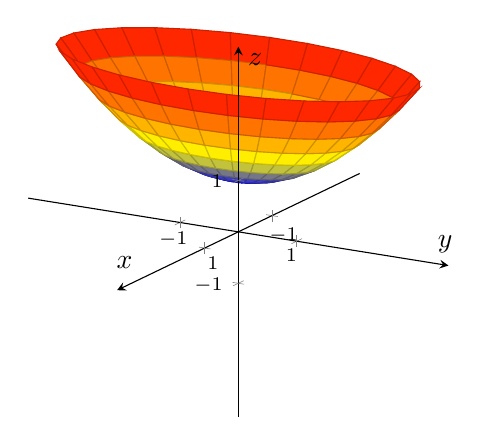
\begin{tikzpicture}[baseline=3.5cm]
			\begin{axis}[
			width=10cm, view={120}{20},
			axis on top,
			axis lines=center,
			enlargelimits=.1,
			tick label style={font=\scriptsize},
			ymin=-3, ymax=3, xmin=-3, xmax=3, zmin=-3, zmax=3,
			xlabel=$x$, ylabel=$y$, zlabel=$z$, xtick={-1,1},ytick={-1,1},ztick={-1,1}
			]
			\addplot3[surf,domain=0:360,y domain=0:1.5, ,samples=30,samples y=10,z buffer=sort] ({y*cos(x)},{2*y*sin(x)},{1+y*y});  
			\end{axis}
			\end{tikzpicture}
		\end{solution}
		\begin{workarea}{1.75in}
			Type of surface: \fillin{2in}{elliptic paraboloid} 	\hfill\begin{tikzpicture}[baseline=4cm]
			\begin{axis}[
			width=10cm, view={120}{20},
			axis on top,
			axis lines=center,
			enlargelimits=.1,
			ymin=-3, ymax=3, xmin=-3, xmax=3, zmin=-3, zmax=3,
			xlabel=$x$, ylabel=$y$, zlabel=$z$, xtick=\empty,ytick=\empty,ztick=\empty
			]
			\end{axis}
			\end{tikzpicture}
		\end{workarea}
		\item\PTs{6} $x^2+z^2-4y^2=4\quad$ 
		\begin{solution}[1.75in]
		
				Type of surface: \underline{$\quad$ hyperboloid of one sheet $\quad$}  % % cheap hack; won't do \hfill in solutions (ok in workarea)
						\hspace{3.5cm}
			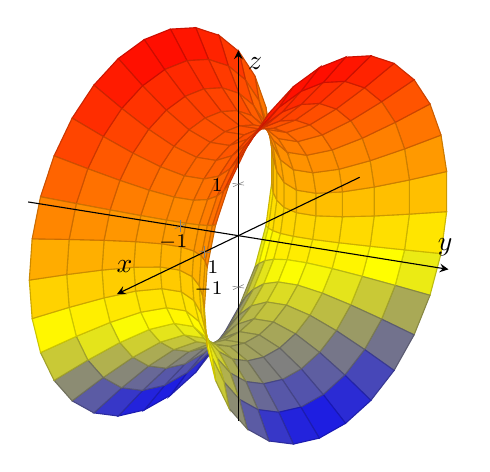
\begin{tikzpicture}[baseline=3.5cm]
			\begin{axis}[
			width=10cm, view={120}{20},
			axis on top,
			axis lines=center,
			enlargelimits=.1,
			tick label style={font=\scriptsize},
			ymin=-3, ymax=3, xmin=-3, xmax=3, zmin=-3, zmax=3,
			xlabel=$x$, ylabel=$y$, zlabel=$z$, xtick={1},ytick={-1},ztick={-1,1}
			]
			\addplot3[surf,domain=0:360,y domain=-1.5:1.5,samples=30,samples y=10,z buffer=sort] ({2*sqrt(y*y+1)*cos(x)},{y},{2*sqrt(y*y+1)*sin(x)});  
			\end{axis}
			\end{tikzpicture}
		\end{solution}
		\begin{workarea}{1.75in}
			Type of surface: \fillin{2in}{hyperboloid of one sheet} 	\hfill\begin{tikzpicture}[baseline=4cm]\vspace{-0.2in}
			\begin{axis}[
			width=10cm, view={120}{20},
			axis on top,
			axis lines=center,
			enlargelimits=.1,
			ymin=-3, ymax=3, xmin=-3, xmax=3, zmin=-3, zmax=3,
			xlabel=$x$, ylabel=$y$, zlabel=$z$, xtick=\empty,ytick=\empty,ztick=\empty
			]
			\end{axis}
			\end{tikzpicture}
		\end{workarea}
%		\item\PTs{5} $x^2+y^2+z^2+2x-4y=4$
%		\begin{solution}[1.75in]
			
%			\hspace{9.15cm}\begin{tikzpicture}
%			\begin{axis}[
%			width=10cm, view={120}{20},
%			axis on top,
%			axis lines=center,
%			enlargelimits=.1,
%			tick label style={font=\scriptsize},
%			ymin=-3, ymax=3, xmin=-3, xmax=3, zmin=-3, zmax=3,
%			xlabel=$x$, ylabel=$y$, zlabel=$z$, xtick={1,2,3},ytick={1,2,3},ztick={1,2,3},
%			xticklabel={${\pgfmathparse{int(2*\tick)}\pgfmathresult}$},yticklabel={${\pgfmathparse{int(2*\tick)}\pgfmathresult}$},zticklabel={${\pgfmathparse{int(2*\tick)}\pgfmathresult}$}
%			]
%			\addplot3[blue] coordinates % % rescaled by half
%			{ (3,0,0)  (0,1.5,0) (0,0,1) (3,0,0)}; 
%			\addplot3[domain=-1/3:1.5, y domain=-0.5:3.2,surf,samples=2,samples y=2,shader=flat,blue!50,opacity=0.5] (y,{1.5-1.5*x-0.5*y},x); 
%			\end{axis}
%			\end{tikzpicture}
%		\end{solution}
%		\begin{workarea}{1.75in}
%			Type of surface: \fillin{2in}{sphere} \hfill\begin{tikzpicture}[baseline=4cm]
%			\begin{axis}[
%			width=10cm, view={120}{20},
%			axis on top,
%			axis lines=center,
%			enlargelimits=.1,
%			ymin=-3, ymax=3, xmin=-3, xmax=3, zmin=-3, zmax=3,
%			xlabel=$x$, ylabel=$y$, zlabel=$z$, xtick=\empty,ytick=\empty,ztick=\empty
%			]
%			\end{axis}
%			\end{tikzpicture}
%		\end{workarea}
	\end{parts}
\end{problem*}

%--------------------------Problem 9----------------------------
\begin{problem}[12] A particle is moving in space from an initial position $\mathbf{r}(0)=\avec{0,0,1}$ and initial velocity $\mathbf{v}(0)=\avec{2,1,2}$ according to the following  \textbf{\emph{acceleration}} (measured in ft/s) at time $t$:
	$$\mathbf{a}(t)=\avec{4e^{2t},6t,\dfrac{1}{(t+1)^2}} \qquad,\qquad t \ge 0. $$
	Find the position of the particle at $t=1$ s.
	
	\begin{solution}[3in] 
	\begin{itemize}
	\item $\mathbf{v}(t)=\dsp\int \mathbf{a}(t)\;dt=\avec{2e^{2t},3t^2,\dfrac{-1}{t+1}}+\mathbf{c} $
	\item $\avec{2,1,2}=\mathbf{v}(0)=\avec{2,0,-1}+\mathbf{c} \quad\Rightarrow\quad \mathbf{c}=\avec{2-2,1-0,2+1}=\avec{0,1,3} $
	\item $\mathbf{v}(t)=\avec{2e^{2t},3t^2+1,\dfrac{-1}{t+1}+3} $
	\item for the position at $t=1$ s, we can use:
		\begin{align*}
			\mathbf{r}(1)-\mathbf{r}(0)&=\int_0^1\mathbf{v}(t)\;dt =\int_0^1\avec{2e^{2t},3t^2+1,\dfrac{-1}{t+1}+3}\;dt=\Big[\avec{e^{2t},t^3+t,3t-\ln(t+1)}\Big]_{0}^{1}\\
			\Longleftrightarrow\quad \mathbf{r}(1)-\avec{0,0,1}&=\avec{e^{2},2,3-\ln(2)}-\avec{1,0,0}\\
			\Longleftrightarrow\quad \mathbf{r}(1)&=\avec{e^{2}+0-1,2+0-0,3-\ln(2)+1-0}\quad\Longleftrightarrow\quad \boxed{\mathbf{r}(1)=\avec{e^{2}-1,2,4-\ln(2)}.}
			\end{align*}
	\end{itemize}

	
	\end{solution}
\end{problem}

%--------------------------Problem 8-----------------------------------------------
\begin{problem}[6] Let $f(t)=\dfrac{1}{t}$ and let $\mathbf{r}(t)=\avec{t^2-1,\tan t}.$ Compute the derivative $\dfrac{d}{dt}\left[f(t)\mathbf{r}(t)\right]$ by using the rules of differentiation for a product. No credit will be given for substituting first.

		\begin{solution}[2.25in] We have $f'(t)=\dfrac{-1}{t^2}$ and $\mathbf{r'}(t)=\avec{2t,\sec^2t}$.
		
		So, by the product rule
		$$\dfrac{d}{dt}\left[f(t)\mathbf{r}(t)\right]=f'(t)\mathbf{r}(t)+f(t)\mathbf{r'}(t)=\dfrac{-1}{t^2}\avec{t^2-1,\tan t}+\frac{1}{t}\avec{2t,\sec^2t}=\avec{-1+\dfrac{1}{t^2},\dfrac{-\tan t}{t^2}}+\avec{2,\dfrac{\sec^2t}{t}} $$
		$$\boxed{\dfrac{d}{dt}\left[f(t)\mathbf{r}(t)\right]=\dfrac{1}{t^2}\avec{t^2+1,t\sec^2t-\tan t}} $$
		\end{solution}

\end{problem}

		


%-------------------------Problem 5--------------------------

\begin{problem*}[6] Physical applications. Choose \emph{one} of the following problems to solve. You may do the other for extra credit only.
	
	\begin{parts}
		\item Find the work done by gravity if a child on a sled with combined weight $60$ lbs goes down $50$ feet along a $30^\circ$ incline.
		
		\begin{solution}[1.75in]
		\begin{center}
		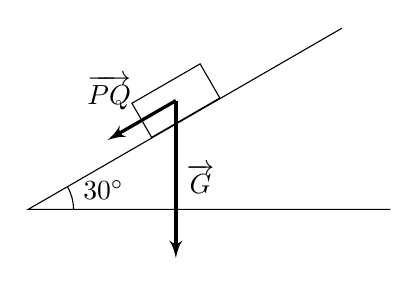
\begin{tikzpicture}[xscale=-1] % % flip image with xscale=-1
		\begin{scope}[scale=1.15]
		\draw (-4,2) -- (0,2) -- +(150:4cm)
		      (-0.5,2) node[above right] {$30^\circ$} arc (180:150:0.5cm);
		      \end{scope}
		      \begin{scope}[rotate=-30]
		      % %for a cart with wheels
		 %     \coordinate (p) at ($sqrt(3)*(-2,0)+(0,2.5)$);
		%\draw ($(p)+(-0.5,-.3)$)  rectangle +(1,0.5);
		%\draw[fill=white] ($(p)+(-0.28,-.35)$) circle (.15 cm);
		%\draw[fill=white] ($(p)+(0.28,-.35)$) circle (.15 cm);
		%\draw[very thick,-latex'] ($sqrt(3)*(-2,0)+(0,2.5)$) -- node[above] {$\vect{F}$} +(-1,0); 
		%\draw[very thick,-latex'] ($sqrt(3)*(-2,0)+(0,2.5)$) -- node[left] {$\vect{G}$} +(300:2cm);
		% OLD PICTURE: cart on hill directly
		      \coordinate (p) at ($sqrt(3)*(-2,0)+(0,2.25)$);
		\draw ($sqrt(3)*(-2,0)+(-0.5,2)$)  rectangle +(1,0.5);
		\draw[very thick,-latex'] ($sqrt(3)*(-2,0)+(0,2.25)$) -- node[above left] {$\vect{PQ}$} +(1,0); 
		\draw[very thick,-latex'] ($sqrt(3)*(-2,0)+(0,2.25)$) -- node[right] {$\vect{G}$} +(300:2cm);
		\end{scope}
		\end{tikzpicture}
		\end{center}
		The angle between $\vect{PQ}$ and the weight from gravity $\vect{G}$ is $60^\circ$. And so we have:
		$$W=\vect{G}\cdot \vect{PQ}=\norm{\vect{G}}\norm{\vect{PQ}}\cos 60^\circ=60(50)\left(\dfrac{1}{2}\right)=\boxed{1500 \text{ ft-lbs}}.$$
		Alternately, set up $\vect{G}=<0,-60>$ and $\vect{PQ}=\avec{50\cos 210^\circ,50\sin210^\circ}=\avec{-25\sqrt{3},-25}$ and do the dot product from the components.
		
			
		\end{solution}
		
		\item Find the magnitude of the torque when applying a force of 10 N directly upwards on a 20-cm wrench that makes a $45^\circ$ angle with the horizontal. 
		
		
		\begin{solution}[1in]
			\begin{center}
			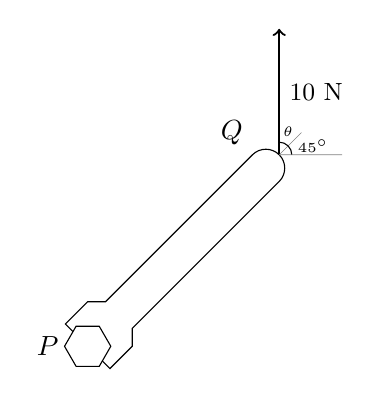
\begin{tikzpicture}
			\begin{scope}[rotate=-45,scale=0.8]
			\draw (0,-2) -| (-0.5,-1.5) -- (-.3,-1.3) -- (-.3,2) arc (180:0:0.3cm) -- (.3,-1.3) -- (0.5,-1.5) |- (0,-2);
			\node[regular polygon, regular polygon sides=6, draw,fill=white,
			inner sep=0.18cm] (b) at (0,-2) {};
			\draw[thick,->] (0,2.3) -- node[right] {\small{10 N}} +(135:2cm) ;
			\draw[help lines] (0,2.3) -- +(0,0.5);
			\draw (0,2.5)  node[right] {\tiny$45^\circ$} arc (90:45:0.2cm);
			\draw (0,2.5) node[above] {\tiny$\theta$} arc (90:135:0.2cm);
			\draw[help lines] (0,2.3) -- +(45:1cm);
			\draw (b) node[left=7pt] {$P$};
			\draw (-.3,2) node[above left] {$Q$};
		%	\draw[blue,thick,fill=white] (b) circle (5pt);
		%	\begin{scope}
		%	\clip (b) circle (5pt);
		%	\draw[thick,blue] ($(-1,1)+(b)$) -- +(2,-2)
		%	      ($(-1,-1)+(b)$) -- +(2,2);
		%	\end{scope}
		%	\draw[thick,blue,->] ($(b)+(165:0.5cm)$) arc (165:-70:0.5cm);
			\end{scope}
		%	\draw (8,-0.5) node[text width=10cm] {$\text{\boldmath$\tau$}=\mathbf{r}\times\mathbf{F}$; by the right hand rule, {\boldmath$\tau$} points towards in the page. Its magnitude is: $\tau=\norm{\mathbf{r}}\norm{\mathbf{F}}\sin\theta=0.2(50)\sin 60^\circ=10\dfrac{\sqrt{3}}{2}=5\sqrt{3}$ Nm.};
			\end{tikzpicture}
			\end{center}
			The magnitude of the torque is:
			$$\tau=\norm{\vect{PQ}\times \vect{F}}=\norm{\vect{PQ}}\norm{\vect{F}}\sin\theta=0.2(10)\sin 45^\circ=2\dfrac{\sqrt{2}}{2}=\boxed{\sqrt{2} \text{ Nm} }.$$
		Alternately, set up $\vect{F}=\avec{0,10,0}$ and $\vect{PQ}=\avec{0.2\cos45^{\circ},0.2\sin45^{\circ},0}=\avec{\dfrac{\sqrt{2}}{10},\dfrac{\sqrt{2}}{10},0}=\dfrac{\sqrt{2}}{10}\avec{1,1,0}$ then,
		$$\vect{\tau}=\vect{PQ}\times\vect{F}=\dfrac{\sqrt{2}}{10}\begin{vmatrix}
		\mathbf{i} & \mathbf{j} & \mathbf{k}\\
		1 & 1 & 0\\
		0 & 10 & 0
		\end{vmatrix}=\dfrac{\sqrt{2}}{10}\avec{0,0,10}=\sqrt{2}<0,0,1>=\sqrt{2}\mathbf{k} $$
		and so the norm of the torque is $\sqrt{2}$ Nm.
		\end{solution}
		
	\end{parts}
	
\end{problem*}


	





\end{exam}
\end{document}
